\documentclass[10pt,twocolumn]{article}
\usepackage[margin=0.6in]{geometry}
\usepackage{graphicx,booktabs,amsmath,hyperref,microtype}
\setlength{\columnsep}{0.22in}\setlength{\parindent}{0pt}\setlength{\parskip}{3pt}
\title{\vspace{-1.2em}RL-Based Smart Elevator Scheduling with a Factorised Double DQN}
\author{J.\ Arjun Naik (B23CM1018)\\GitHub: \url{https://github.com/Mico1704/RL-Based-Smart-elevator-scheduling}}
\date{}
\begin{document}\maketitle\vspace{-1.6em}
\section{Problem and environment}
A central agent controls 3 cars in a 10-floor building (capacity 8) to cut passenger waiting time and energy. Our custom Gymnasium simulator draws Poisson arrivals with pattern-specific rates and origin/destination mixes (up-peak, down-peak, lunch, quiet); an episode is 200 ticks. One tick moves a car one floor or opens its doors (unload, then board FIFO). Energy per car-tick: 1 per floor moved, +0.5 per start, +0.5 per stop; idling is free.
\section{RL formulation}
\textbf{State} ($\mathbb{R}^{137}$). Per car: one-hot floor (10), direction, load, in-car buttons (10), and 12 relational features (pickup/drop target here, nearest below/above with distance, whether another car is closer). Building: per floor up/down call counts and oldest-call age (30), traffic-pattern one-hot (4), time fraction (1).\\
\textbf{Action.} Per car \{down, stop, up\}; joint space $3^3=27$.\\
\textbf{Reward.} $r_t=-\kappa\,(N^{wait}_t+\beta N^{ride}_t)-\lambda E_t$ with $\kappa=0.1$, $\beta=0.25$, $\lambda=0.1$; $E_t$ is the step's energy.\\
\textbf{Algorithm.} Double DQN written in NumPy, with a value-decomposed head $Q(s,\mathbf a)=\sum_{i=1}^{3}Q_i(s,a_i)$ so the 27-way argmax splits into three. MLP 128-128, Adam (3e-4), 8-step returns, $\gamma=0.95$, soft target updates, 250k steps on mixed traffic. Plain one-step DQN collapsed to idling (it ``saved'' energy by never boarding anyone); n-step returns, relational features and \emph{guided exploration} (30--80\% of early episodes driven by a noisy Nearest-car/SCAN controller, learning only from reward) fixed this.
\section{Baselines and evaluation}
Random, Nearest-car (each call to the closest car with room) and SCAN-style (sweep and reverse). All controllers use the same 20 unseen seeds per pattern. Waiting time counts still-queued passengers' current age.
\begin{table}[h]\centering\scriptsize\setlength{\tabcolsep}{2.5pt}
\begin{tabular}{llrrr}\toprule Pattern & Controller & Avg wait & Max wait & Energy\\\midrule
up-peak & Random & 47.4$\pm$9.4 & 128.1$\pm$20.3 & 555.3$\pm$22.3\\
up-peak & Nearest-car & 3.9$\pm$0.8 & 17.2$\pm$4.1 & 355.8$\pm$29.8\\
up-peak & SCAN-style & 4.2$\pm$0.8 & 15.8$\pm$3.9 & 532.5$\pm$20.1\\
up-peak & DQN & 25.3$\pm$15.2 & 90.7$\pm$39.3 & 272.6$\pm$88.4\\
\midrule
down-peak & Random & 37.6$\pm$9.9 & 151.7$\pm$20.8 & 557.7$\pm$17.5\\
down-peak & Nearest-car & 4.1$\pm$0.8 & 25.1$\pm$10.8 & 406.2$\pm$34.8\\
down-peak & SCAN-style & 6.4$\pm$0.9 & 22.3$\pm$3.1 & 575.5$\pm$11.1\\
down-peak & DQN & 19.4$\pm$13.4 & 94.2$\pm$43.9 & 370.1$\pm$84.9\\
\midrule
lunch & Random & 34.7$\pm$5.9 & 137.3$\pm$22.5 & 554.6$\pm$16.3\\
lunch & Nearest-car & 3.2$\pm$0.3 & 15.8$\pm$4.1 & 465.3$\pm$32.1\\
lunch & SCAN-style & 5.4$\pm$1.2 & 22.1$\pm$4.7 & 567.8$\pm$10.1\\
lunch & DQN & 12.0$\pm$7.2 & 61.2$\pm$32.0 & 381.1$\pm$60.8\\
\midrule
quiet & Random & 18.9$\pm$8.2 & 70.2$\pm$29.0 & 552.7$\pm$24.4\\
quiet & Nearest-car & 2.7$\pm$0.5 & 7.4$\pm$2.5 & 139.7$\pm$32.7\\
quiet & SCAN-style & 3.1$\pm$0.5 & 8.3$\pm$2.8 & 259.2$\pm$47.5\\
quiet & DQN & 17.3$\pm$9.1 & 81.0$\pm$36.5 & 134.9$\pm$42.5\\\\\bottomrule\end{tabular}
\caption{Mean $\pm$ std over 20 seeds (time in ticks).}\end{table}
\begin{figure*}[t]\centering
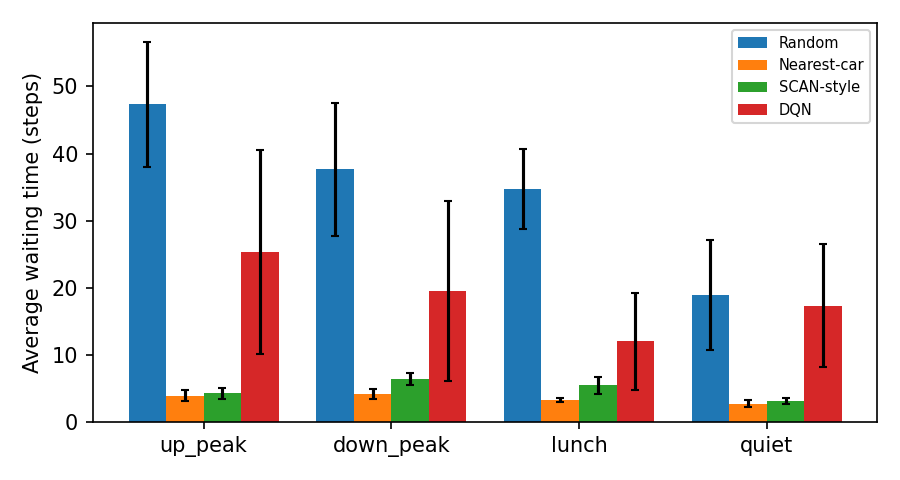
\includegraphics[width=0.245\textwidth]{avg_wait.png}\hfill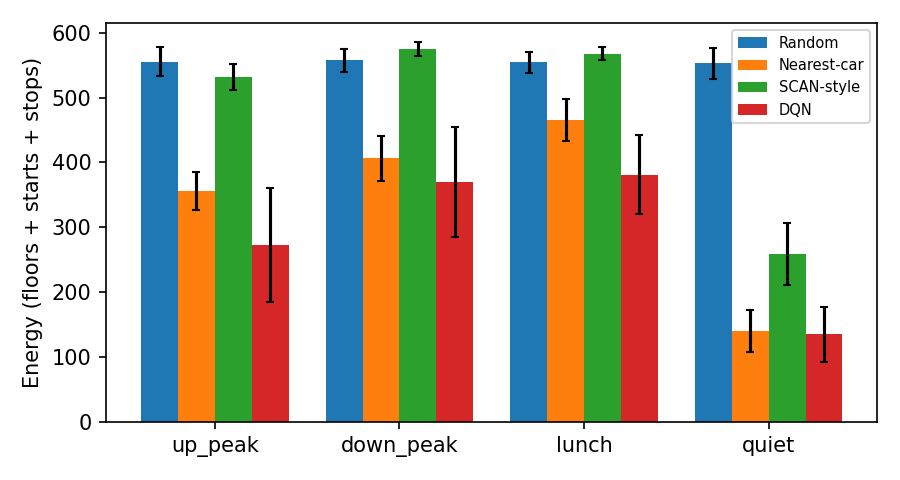
\includegraphics[width=0.245\textwidth]{energy.png}\hfill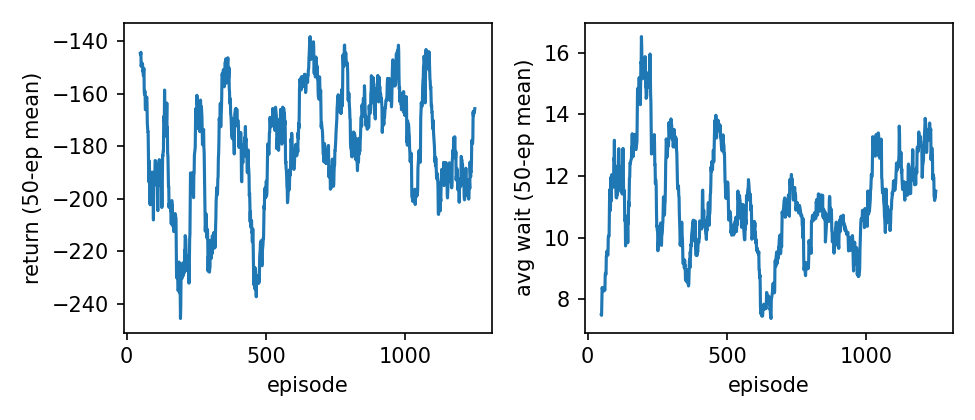
\includegraphics[width=0.245\textwidth]{training_curve.png}\hfill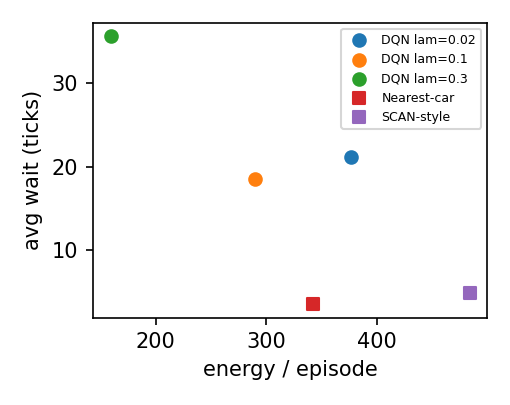
\includegraphics[width=0.2\textwidth]{lambda_tradeoff.png}
\caption{Average wait, energy per episode, DQN training curve, and $\lambda$ trade-off (mean over all patterns, 20 seeds each).}\end{figure*}
\section{Results and discussion}
\textbf{The agent does not meet the success criterion.} It learned to serve most passengers (vs.\ none for the first version) and uses less energy than Nearest-car in 12--19 of 20 seeds per pattern, but its waiting time is 3--6$\times$ higher (better on only 1 of 80 paired runs), with 5--38 passengers unserved per episode; part of the energy saving comes from that unserved demand. Nearest-car is a strong baseline in this small building. \textbf{$\lambda$ sweep} (DQN, averaged over patterns; Nearest-car in brackets): $\lambda=0.02$: wait 21.2, energy 377; $\lambda=0.1$: 18.5, 290; $\lambda=0.3$: 35.7, 160 (Nearest-car 3.5, 342). Raising $\lambda$ cuts energy but lengthens waits, as designed; no setting reaches Nearest-car's waiting time. Likely causes: sparse credit across a shared team reward, 250k steps, and limited tuning. Longer training, a larger network and per-car credit assignment are future work.
\begin{thebibliography}{9}\small
\bibitem{s} Sutton \& Barto, \emph{Reinforcement Learning: An Introduction}, MIT Press, 2018.
\bibitem{v} van Hasselt et al., Deep RL with Double Q-learning, AAAI 2016.
\bibitem{vd} Sunehag et al., Value-Decomposition Networks, 2017.
\end{thebibliography}
\end{document}
